\laborator{Регрессионный анализ, методы аппроксимации}

\goal ознакомиться с возможностями математического пакета Mathcad при решении задач регрессионного анализа; ознакомиться с процедурами численного решения алгебраических уравнений и систем уравнений, реализованными в данном пакете. 

\subsubsection*{Теория}
Регрессионный анализ --- статистический метод исследования зависимости между зависимой переменной $y$ и одной или несколькими независимыми переменными $x_1$, $x_2$, $...$, $x_n$.
В статистике для оценки силы корреляционной зависимости двух случайных величин используется коэффициент корреляции $r_{xy}$. Определяется он отношением математического ожидания произведения отклонений случайных величин от их средних значений к произведению среднеквадратичных отклонений этих величин:
\begin{equation}
r_{xy}=\dfrac{\dfrac{1}{n} \sum\limits_{i=1}^{n} (x_i-\bar{x}) (y_i-\bar{y}), }{\sigma_x \sigma_y}
\end{equation}
где $\sigma_x$ и $\sigma_y$ --- среднеквадратичные отклонения, определяемые следующим образом:
\begin{equation}
\sigma_x=\sqrt{\dfrac{1}{n} \sum\limits_{i=1}^{n}(x_i-\bar{x})^2},
\end{equation}
где $\bar{x}=\dfrac{1}{n} \sum\limits_{i=1}^{n} x_i$.
Аналогичные выражения записываются и для $y$.

В Mathcad коэффициент корреляции двух выборок по данной формуле можно подсчитать с помощью встроенной функции \mc{corr (x,y)} (где \mc{x} и \mc{y} --- векторы, между которыми определяется коэффициент корреляции). Если коэффициент корреляции равен по модулю единице, то между случайными величинами существует линейная зависимость. Если же он равен нулю, то случайные величины независимы. В случае промежуточных значений $r_{ху}$, зависимость $y$ от $x$ может быть нелинейной или иметь высокое значение шума.

Если две выборки коррелируют, то можно установить зависимость между ними. Для проведения регрессионного анализа в Mathcad имеется ряд функций. Конечный результат регрессионного анализа --- получение функции с набором параметров, с помощью которой можно оценить значения в промежутках между заданными точками. Расхождение полученной функции регрессии с экспериментальными данными можно оценить через относительную среднюю и максимальную ошибку:

\begin{equation}
err_i= \dfrac{\left| y_i^э - y(x^э_i) \right|}{y_i^э} 100\ \% ,
\end{equation}
\begin{equation}
err_{av}=\dfrac{1}{n}\sum\limits_{i=1}^{n} err_i ,
\end{equation}
где $y_i^э$, $y(x_i^э)$ --- экспериментальное и расчетное значения функции; $n$ --- число экспериментальных точек; $err_i$ --- ошибка в i–й точке (из них определяется максимальная); $err_{av}$ --- средняя ошибка функции регрессии.

В Mathcad имеются встроенные функции для определения среднего и максимального значения массива: \mc{mean(S)} находит среднее значение элементов матрицы \mc{S}, \mc{max(S)} --- максимальное значение.

\subsubsection{Линейная регрессия}
Линейная функция $y=ax + b $ является одной из наиболее простых и часто применяется для описания экспериментальных данных. 
Если поместить значения $x$ в вектор \mc{VX} и соответствующие значения $y$ в \mc{VY}, то линейная функция определяется в виде:
\mc{Y = slope(VX, VY) $\cdot$ X + intercept(VX, VY)},
где \mc{slope(VX, VY)} --- возвращает скаляр: тангенс угла наклона линии регрессии для данных из \mc{VX} и \mc{VY} (параметр $a$);
\mc{intercept(VX, VY)} - возвращает скаляр: смещение по оси ординат линии регрессии для данных из \mc{VX} и \mc{VY} (параметр $b$).

%Пример решения
\primer{Задайте экспериментальные данные, близкие к линейной зависимости, в виде таблицы. Определите коэффициент корреляции. Получите функцию линейной регрессии, описывающую эти экспериментальные данные. Графически и численно определите точность полученной функции регрессии.}

\begin{center}
	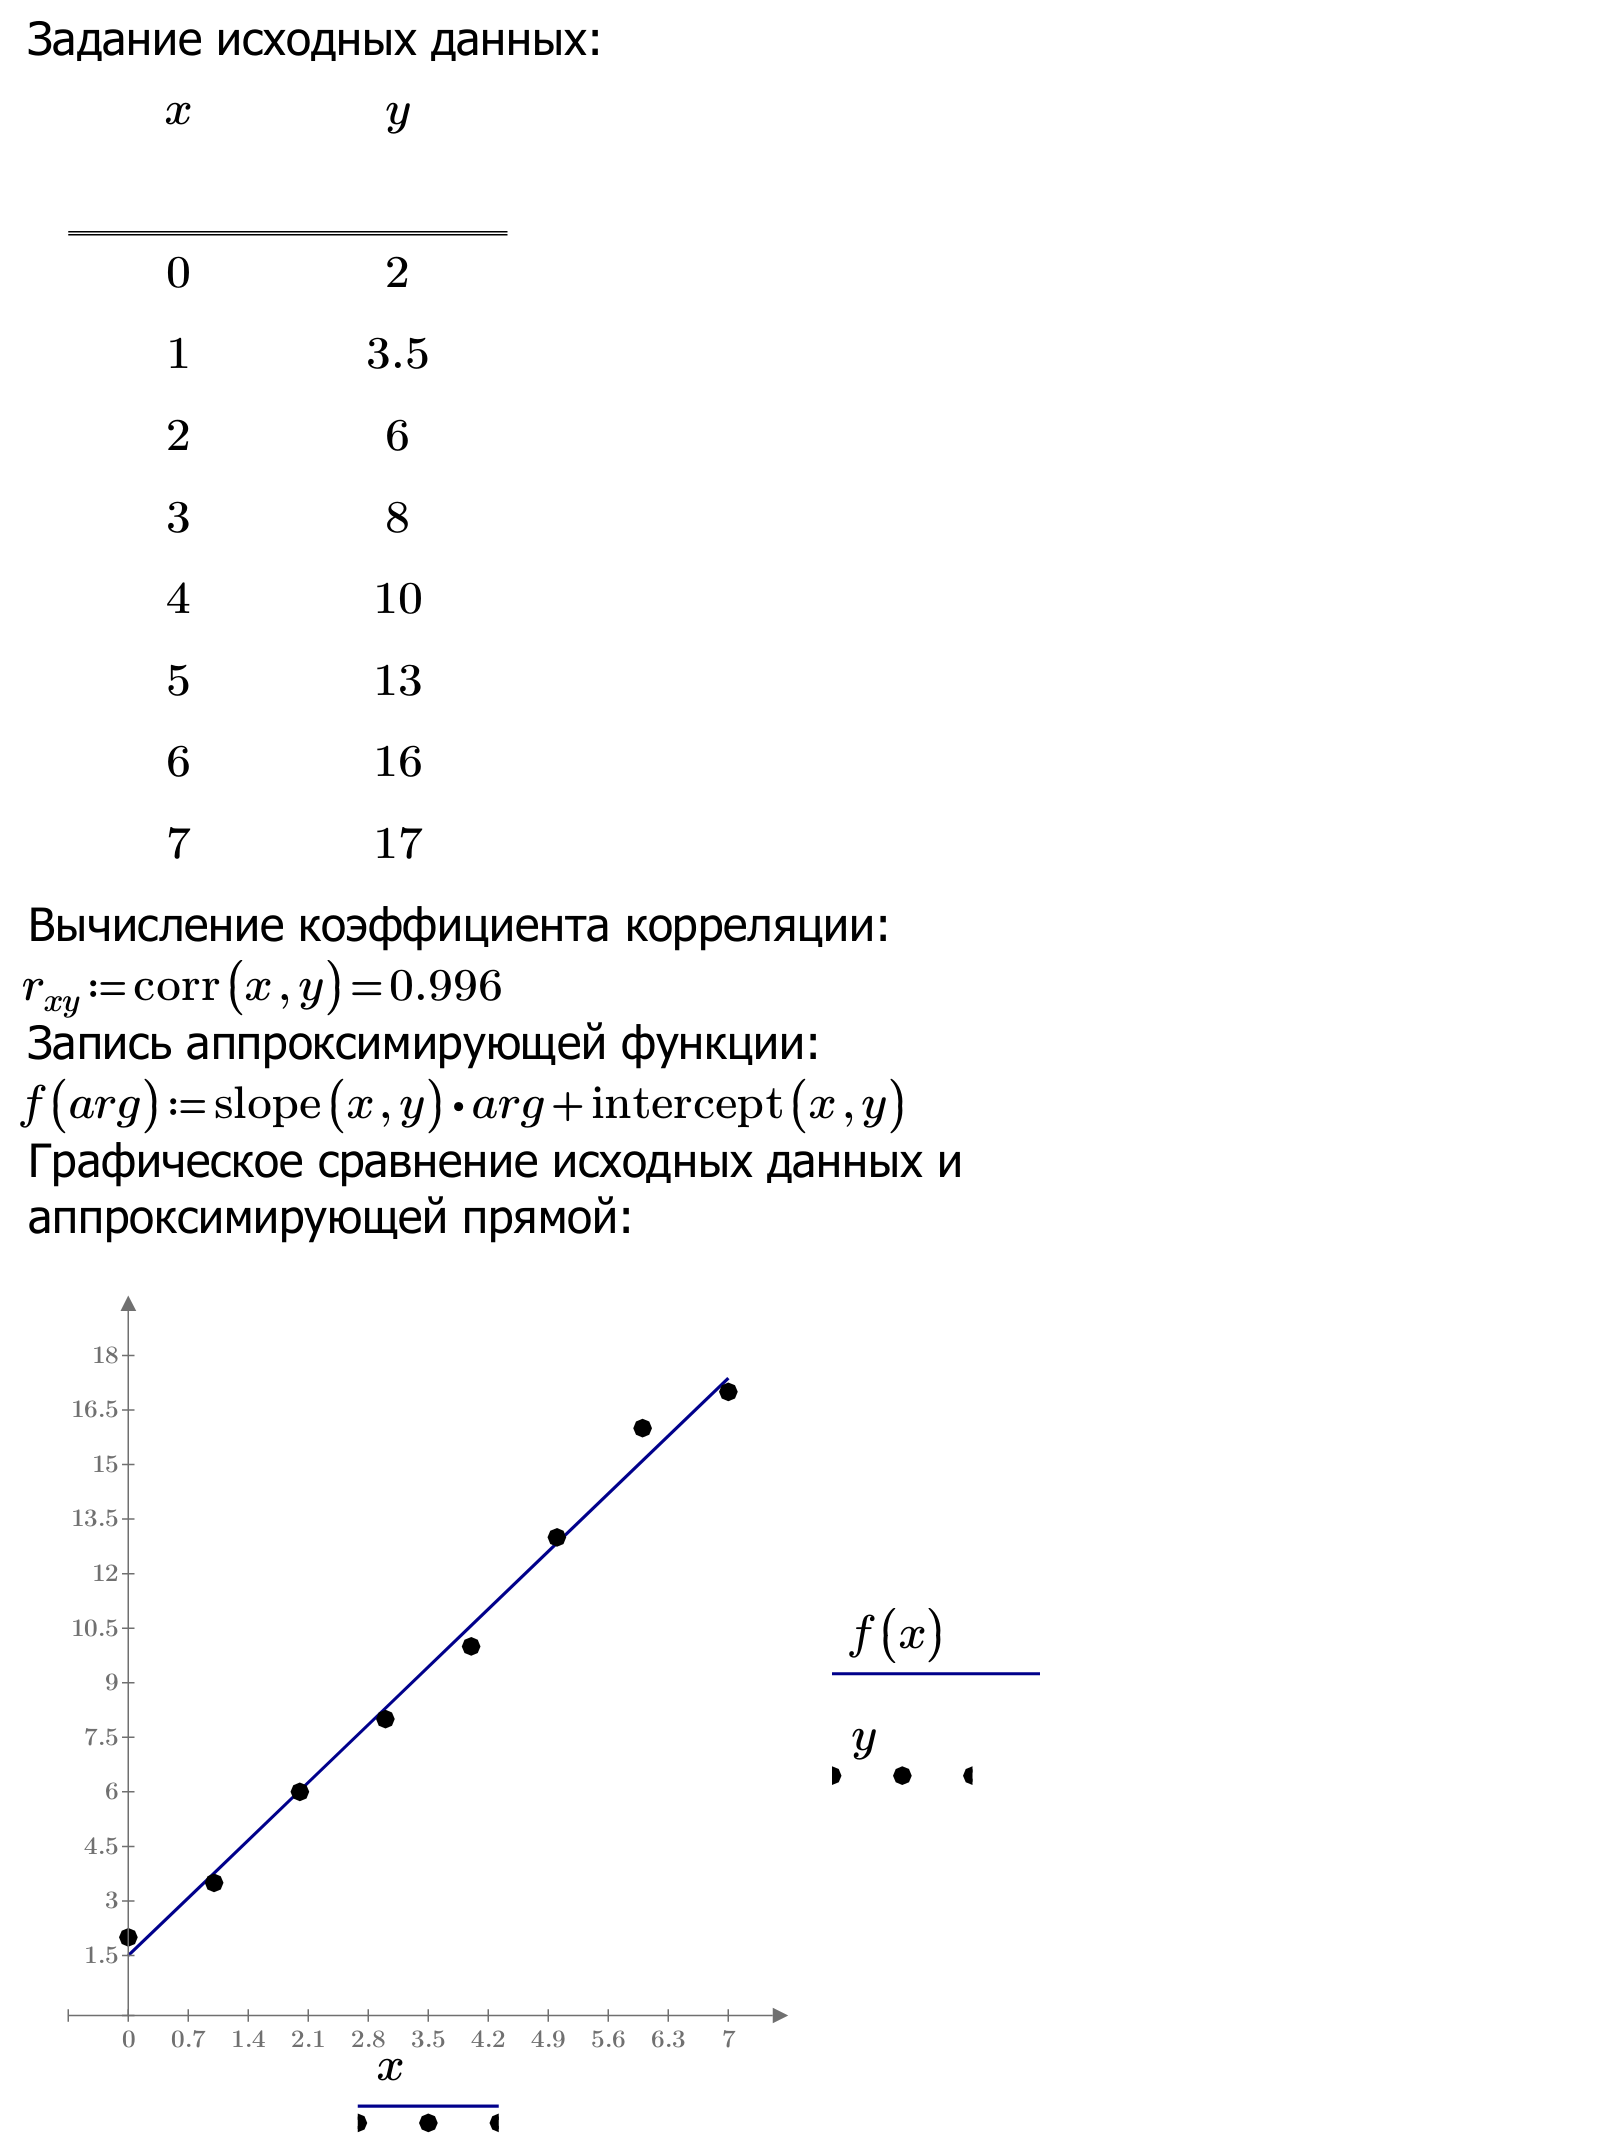
\includegraphics[scale=1.0]{new-regress-1-1.png}
\end{center}
\begin{center}
	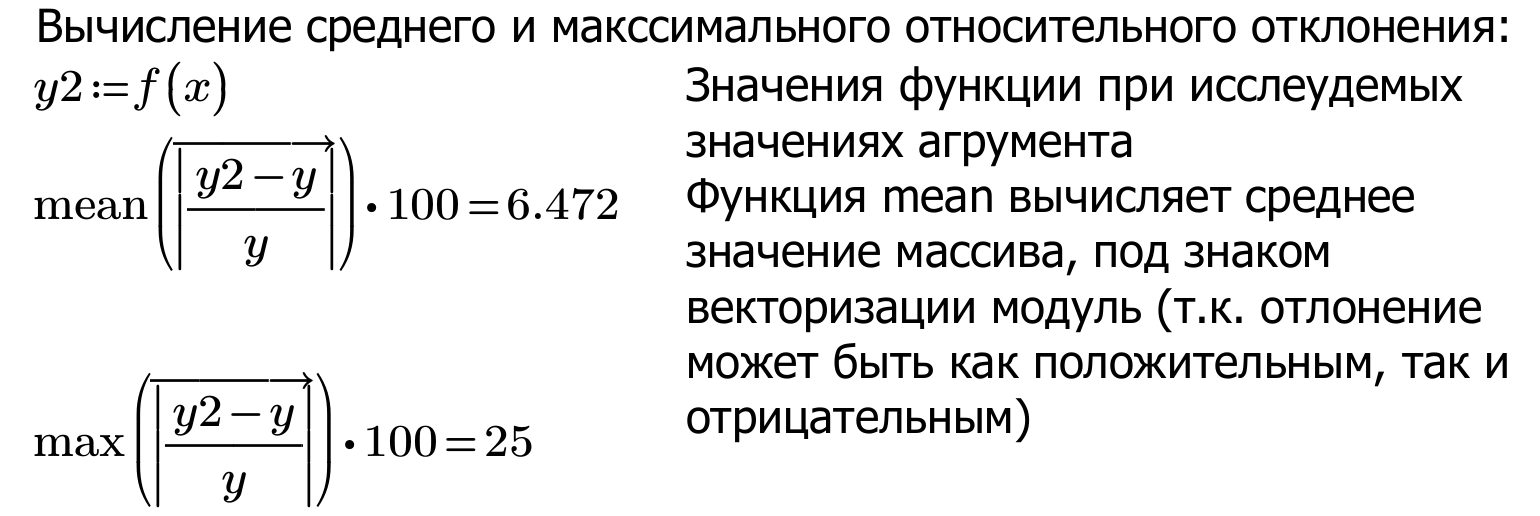
\includegraphics[scale=1.0]{new-regress-1-2.png}
\end{center}

\subsubsection{Полином}
Одной из  часто применяемых при обработке экспериментальных данных функций, является полиномиальная:
\begin{equation}
y(x)= \sum_{i=0}^{n} a_i x^i
\end{equation}
где $a$ --- параметры полинома, $n$ --- степень полинома. Для определения параметров полиномов используется функция \mc{regress}, которая допускает использование полинома любого порядка. Однако на практике не следует использовать степень полинома выше $n = 4$. Так как функция \mc{regress} пытается приблизить все точки данных, при недостаточном количестве экспериментальных данных высокая степень полинома может дать физически неадекватное поведение результирующей функции.

\mc{regress(vx, vy, n)} --- функция, определяющая параметры полином порядка \mc{n}, \mc{vx} и \mc{vy} --- m-мерные векторы, содержащие значения $x$ и $y$. Функция \mc{regress} возвращает вектор, содержащий кроме самих значений параметров полинома $a$ множество технической информации. Для того, чтобы вычислить значение полинома в какой-либо, точке используется функция: \mc{interp (vs, vx, vy, x)} --- возвращает интерполируемое значение $y$, соответствующее $x$.

\primer{Задайте экспериментальные данные в виде таблицы. Определите коэффициент корреляции. На основе этих данных получите функцию полиномиальной регрессии, описывающую экспериментальные данные. Графически и численно определите точность полученной функции регрессии.}

\begin{center}
	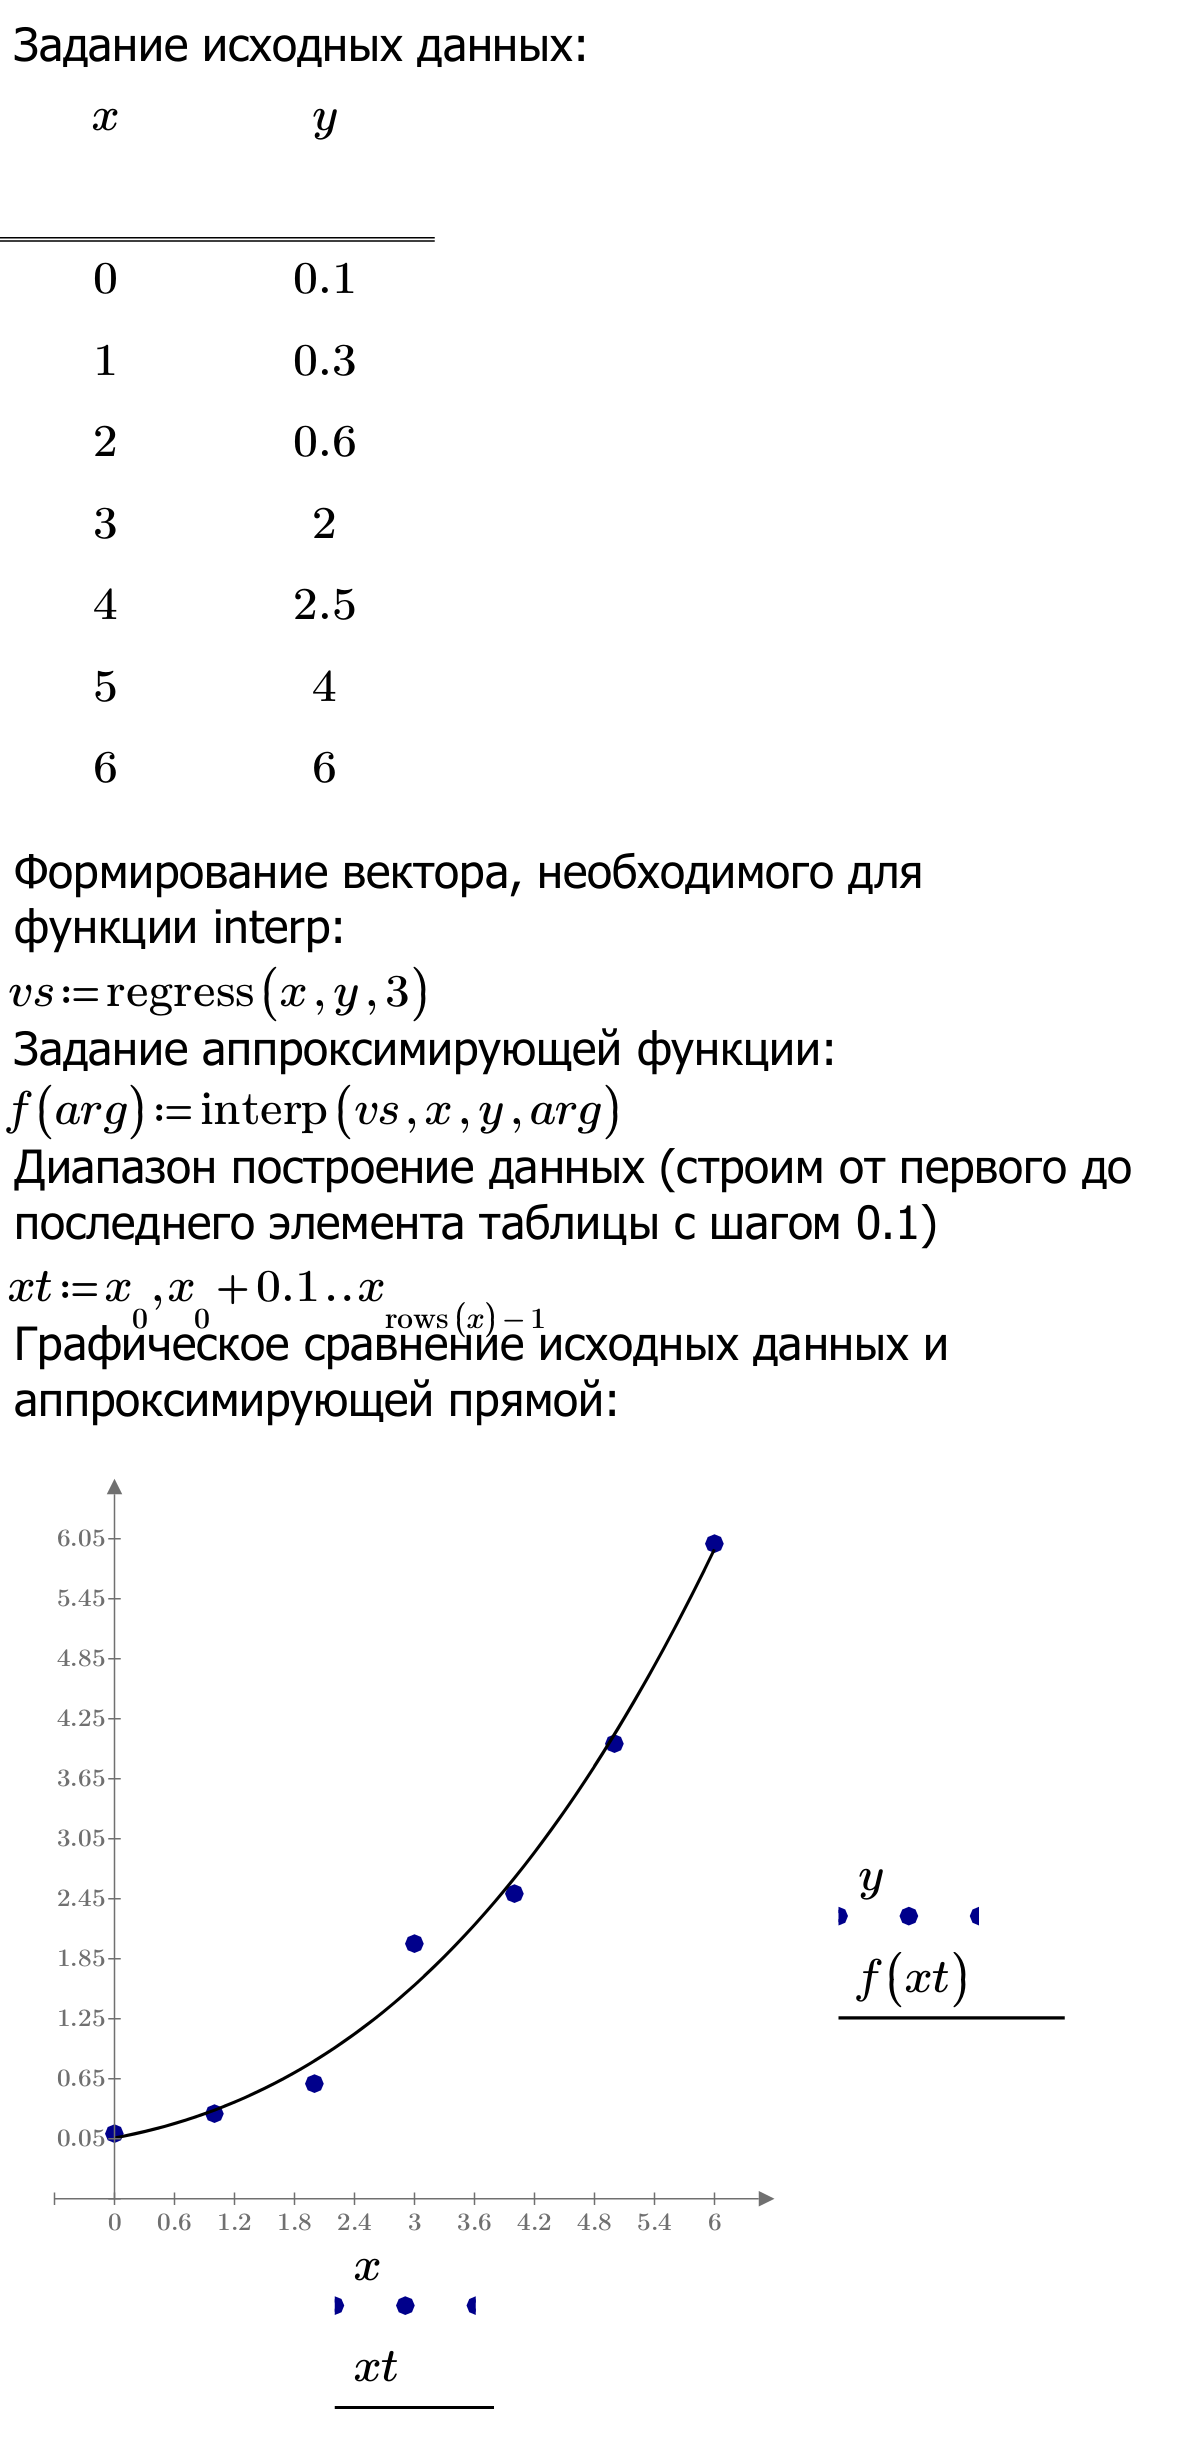
\includegraphics{new-regress-2.png}
\end{center}


\subsubsection{Обобщенная линейная регрессия (линейные по параметрам функции)}
Обобщенная линейная регрессия --- зависимость в виде линейных комбинаций произвольных функций, ни одна из которых не является полиномом.
Задача обобщенной линейной регрессии --- найти, какие значения должны принимать параметры $a_0, a_1, ..., a_N$, чтобы функция  $F(x)=a_0 f_0(x)+a_1 f_1(x)+ ... + a_N f_N(x)$, являющаяся линейным сочетанием $N+1$ произвольной функции $f_i(x)$, проходила между экспериментальными точками так, чтобы сумма квадратов расстояний от точек до кривой $F(x)$ была минимальной.

В Mathcad для вычисления параметров обобщенной линейной регрессии служит встроенная функция \mc{linfit(x, y, F)}, где \mc{x} и \mc{y} --- векторы экспериментальных данных, \mc{F} --- векторная функция, содержащая в качестве элементов функции, входящие в линейное сочетание.

\primer{Задайте произвольный набор данных $y$ и $x$. С помощью функции \mc{linfit} определите вид линейной зависимости между $y$ и $x$. В качестве функции используйте выражение
	$F(x)=a_0 \sin(x) + a_1 \cos(2x)+a_2 \sqrt[3]{x} + a_3 x$.}
%пример решения

\begin{center}
	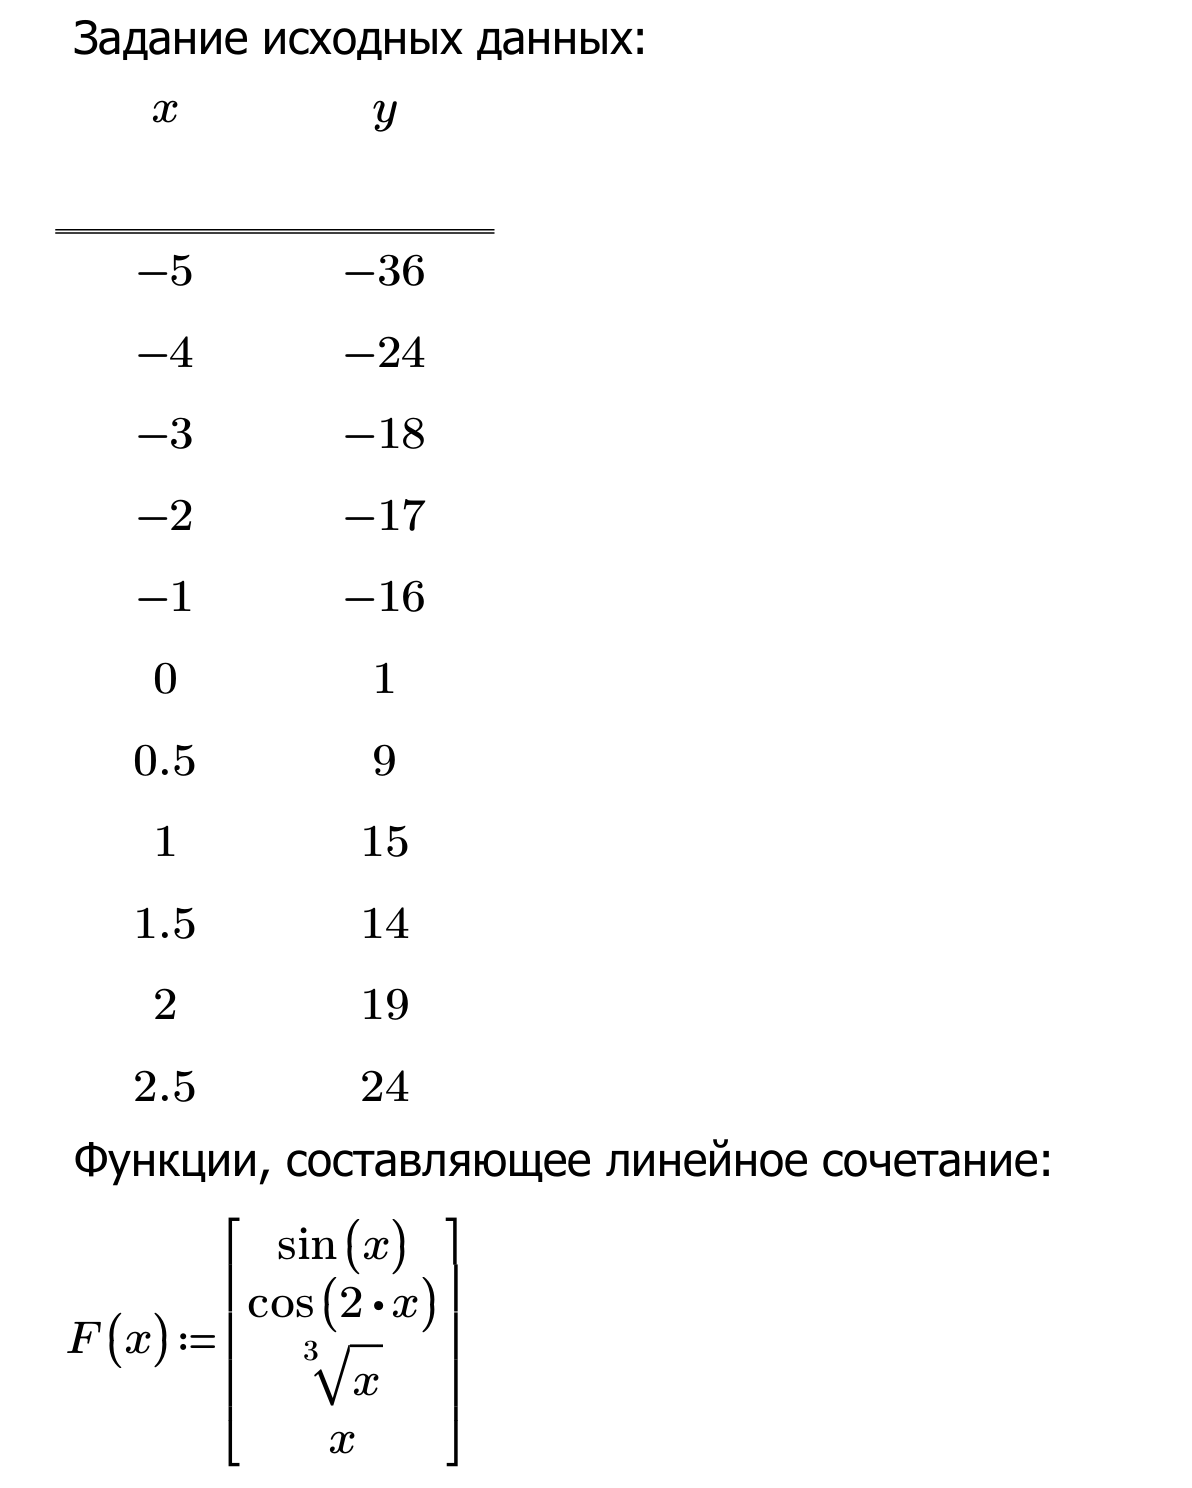
\includegraphics{new-regress-3-1.png}
\end{center}
\begin{center}
	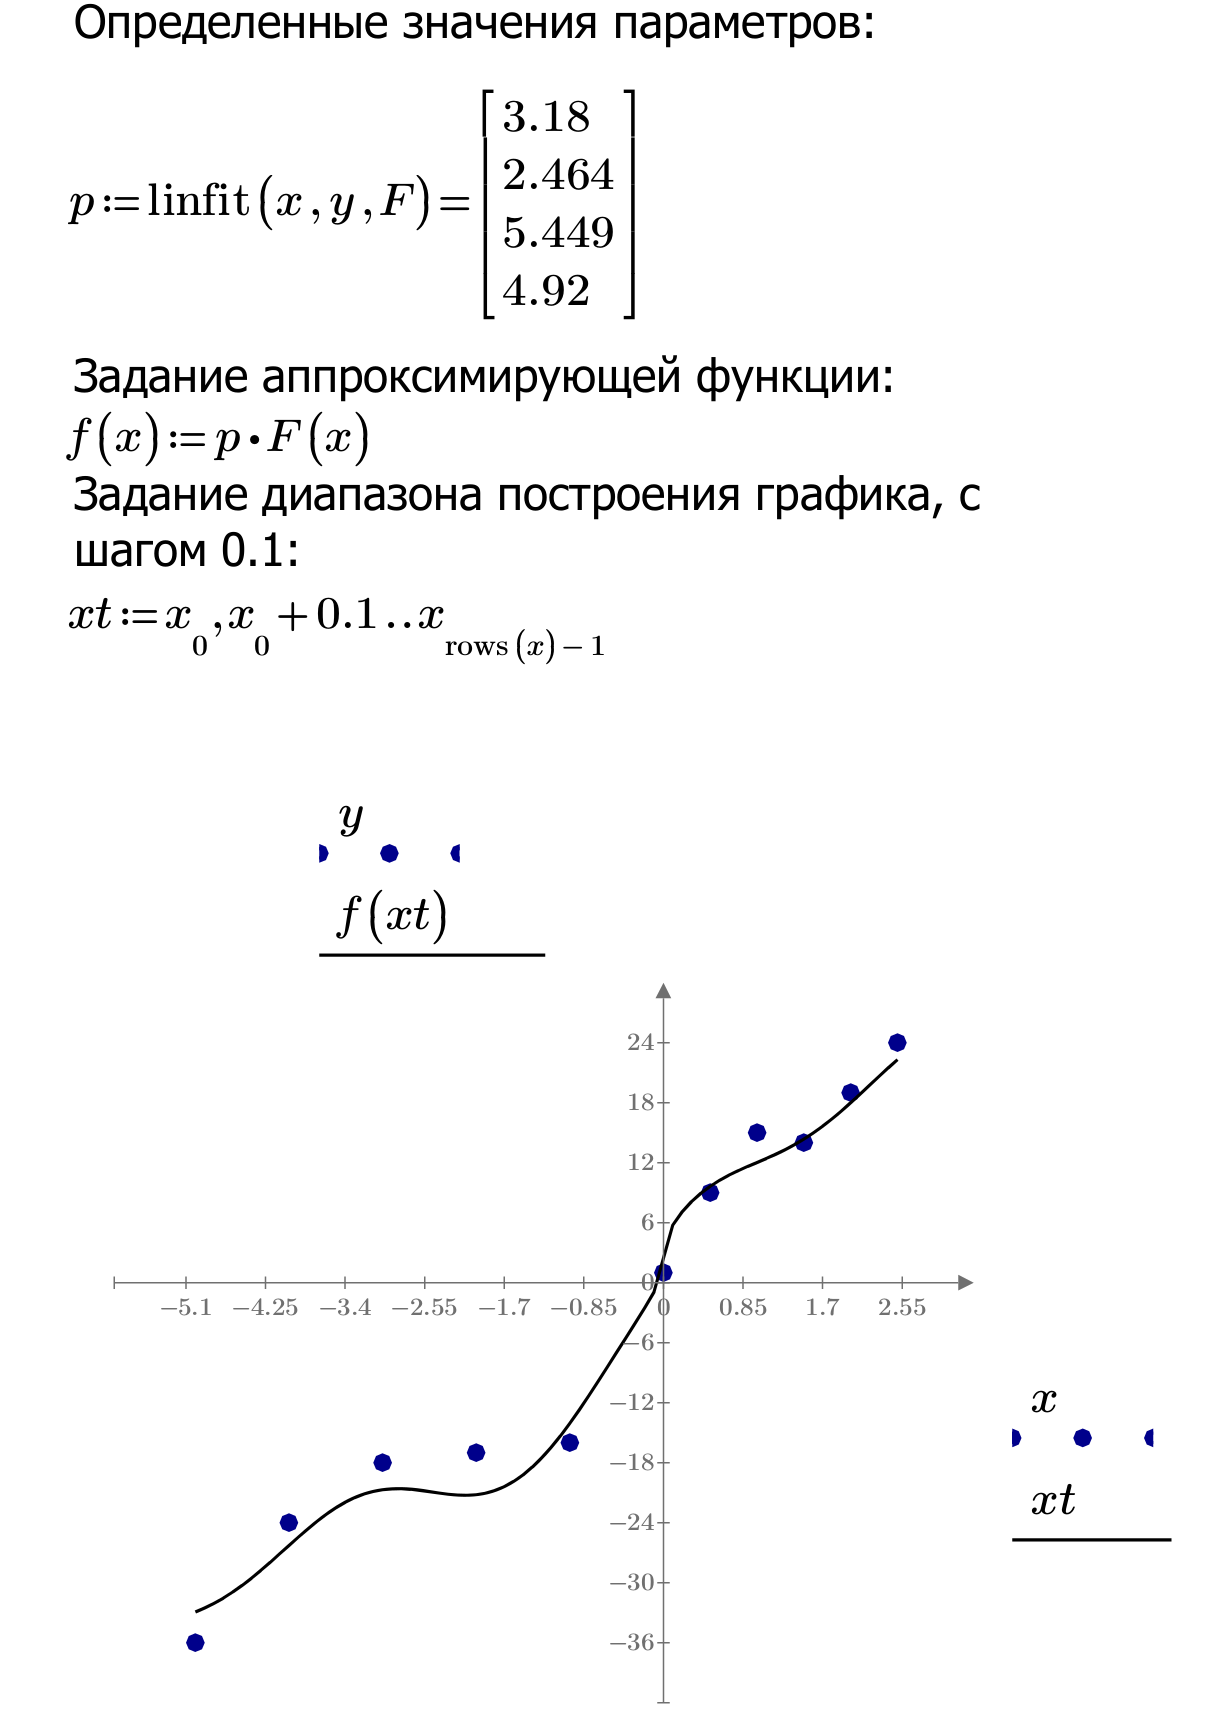
\includegraphics{new-regress-3-2.png}
\end{center}


\subsubsection{Нелинейная регрессия (нелинейные по параметрам функции)}

Если аппроксимирующая исходные данные функция представляется в виде $F(x) = f_0 (a_0, x) + f_1(a_1,x) +... + f_N(a_N,x)$, когда искомые коэффициенты $a_0, a_1, ..., a_N$ входят в функции, зависимость будет уже нелинейной по параметрам, соответственно функция \mc{linfit} уже не подойдет.
В Mathcad заложены зависимости наиболее распространенных нелинейных функций: синуса, экспоненты или др. Параметры для этих нелинейных зависимостей определяются функциями: 
\begin{itemize}
	\item \mc{expfit(x, y, g)} --- регрессия  экспоненциальной функцией $y(x)=a e^{b x}+c$;
	\item \mc{lgsfit(x, y, g)} --- регрессия логистической функцией $y(x)=a/(1+b e^{-c x})$;
	\item \mc{sinfit(x, y, g)} --- синусоидальная регрессия $y(x)=a sin(x+b)+c$;
	\item \mc{pwrfit(x, y, g)} --- регрессия степенной функцией $y(x)=a x^b+c$;
	\item \mc{logfit(x, y, g)} --- регрессия логарифмической функцией $y(x)=a\ln(x+b)+c$;
\end{itemize}
где \mc{g} --- вектор начальных приближений для поиска параметров. 

В случае, если используется какая~-либо произвольная нелинейная регрессия,  в Mathcad есть встроенная функция \mc{genfit(x, y, g, F)}. В качестве аргументов данная функция принимает следующие параметры: \mc{x}, \mc{y} --- вектор экспериментальных данных; \mc{g} --- вектор начальных приближений для неизвестных параметров;
\mc{F(x, A)} --- описывающая экспериментальную зависимость функция, параметры \mc{A} которой должны быть определены.

Параметры \mc{x} и \mc{y} приведенных функций соответствуют векторам координат исходных эмпирических данных. В переменной \mc{g} содержится вектор начальных приближений искомых параметров \mc{(a, b, c)}. Для определения параметров нелинейных по параметрам функций используются различные алгоритмы (например Левенберга~--Марквардта, градиентного спуска и т.д.) данные алгоритмы основаны на использовании каких-либо значений для параметров на первой итерации поиска.
Из всех встроенных функций регрессии \mc{genfit} является наиболее универсальной и может быть использована для любых функций. Однако для нелинейных по параметрам функций огромное влияние на точность расчета оказывает начальное приближение  \mc{g} для искомых параметров. Поэтому при возможности лучше ввести задачу к  использованию линейных по параметрам функции.

\primer{Задайте произвольный набор данных \mc{x} и \mc{y} в виде таблицы. Определите коэффициент корреляции между данными. Для аппроксимации данных используете функцию вида $y(x)=\exp(A+Bx+Cx^2)$ где $A$, $B$, $C$ --- параметры. Оценить точность полученной регрессии.}
%пример решения

\begin{center}
	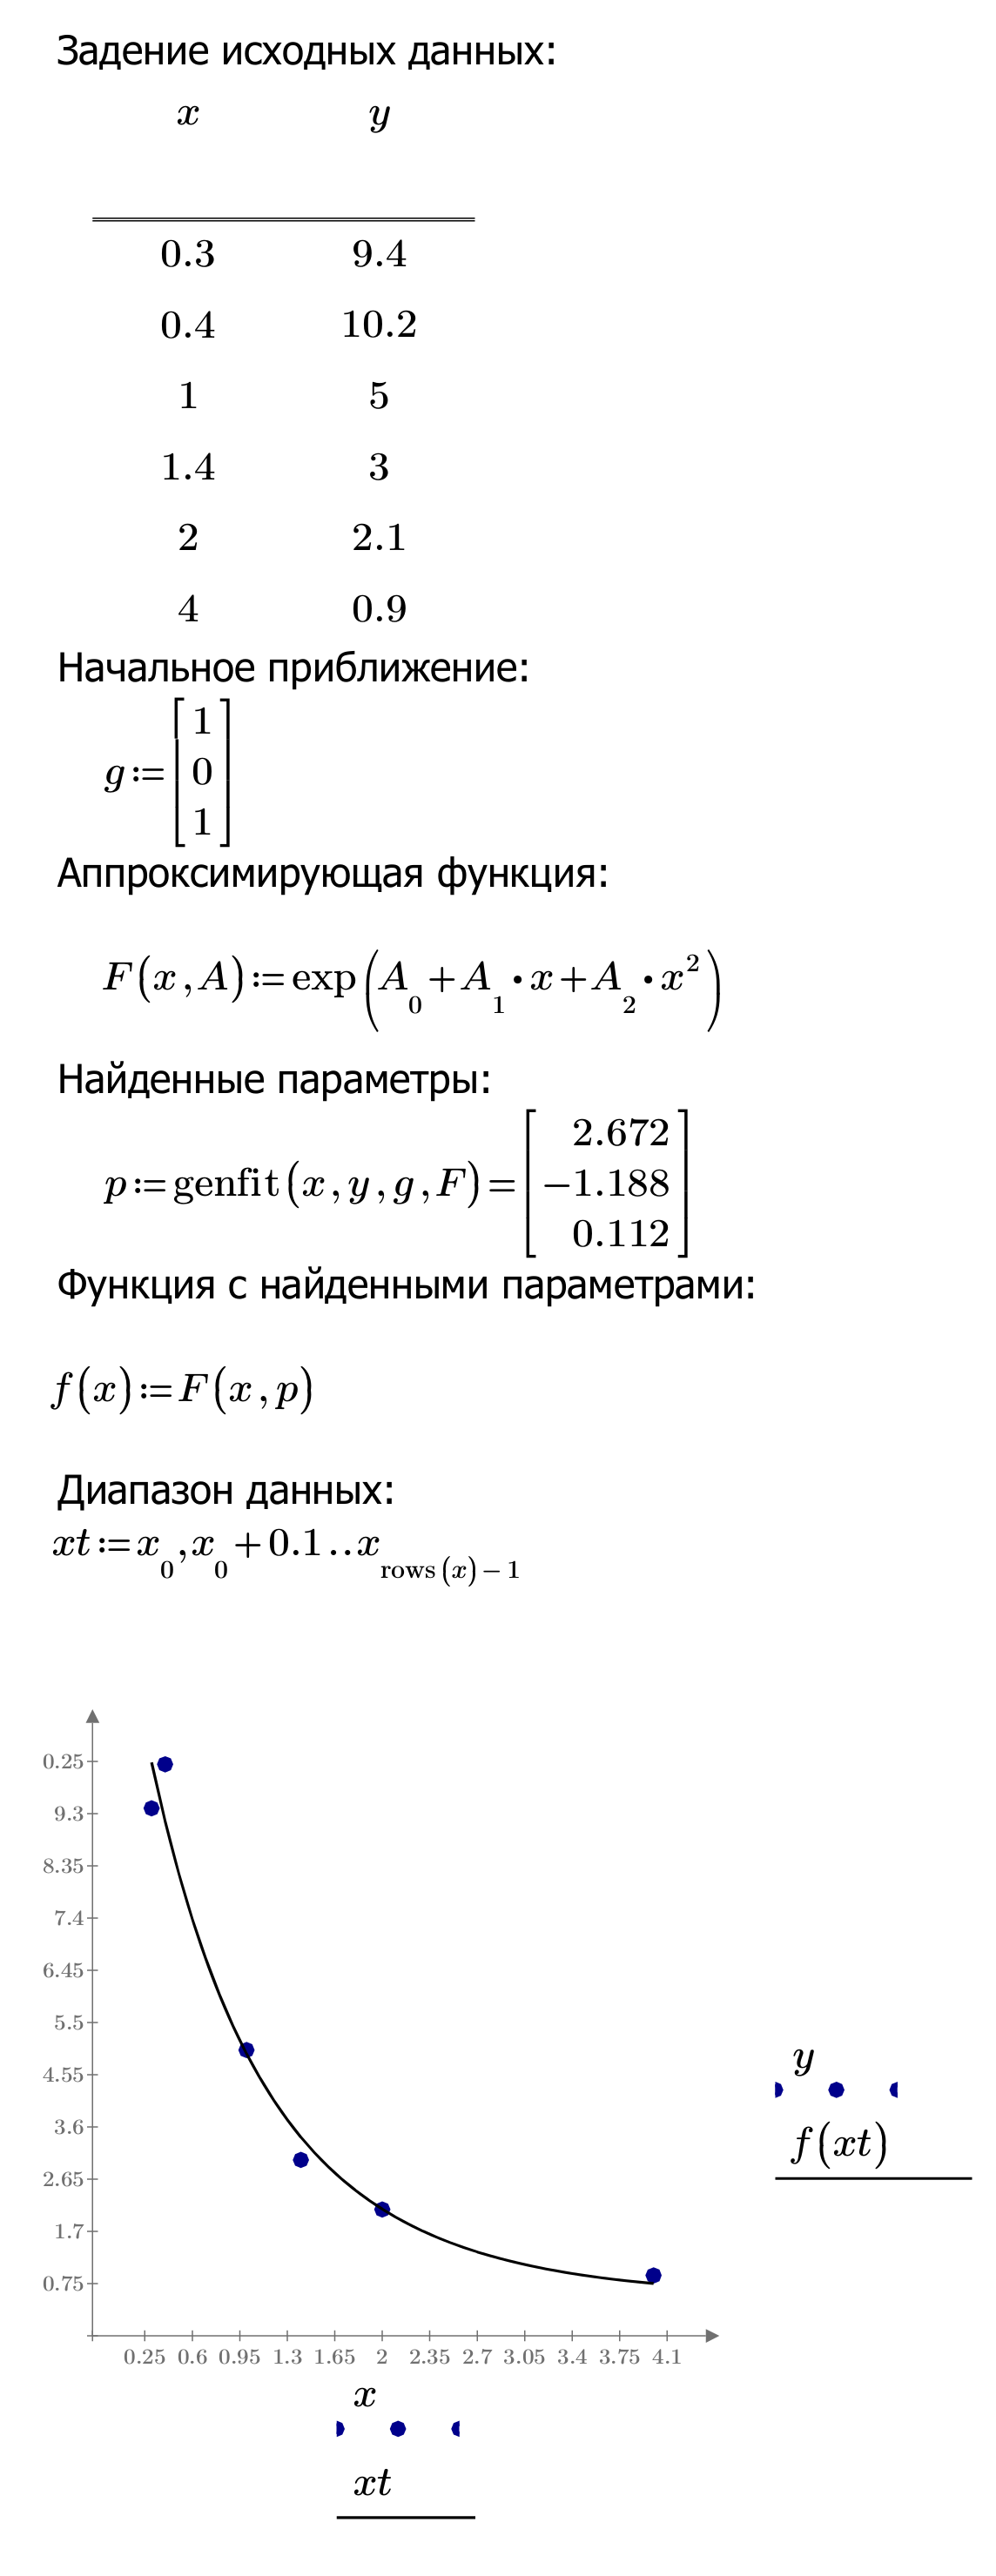
\includegraphics{new-regress-4.png}
\end{center}

В случае обработки точных данных, представленных в дискретном виде удобнее использовать сплайны. Сплайн представляет из себя кусочную функцию, составленную из полиномов какой-либо степени. Границы использования полиномов начинаются и заканчиваются строго во введенных значениях точек $x$ и $y$ (рисунок \ref{fig:old.regress.spline}). Также параметры полиномов настраиваются таким образом, что производная двух полиномов с каждой из сторон подходящих к точке будет одинаковой.
Таким образом два этих условия обеспечивают непрерывность и гладкость (непрерывность производной) сплайна. Однако сплайны неприемлемо применять для аппроксимации экспериментальных данных в связи с тем, что погрешности эксперимента будут вносить существенное влияние на результирующую функцию. В представленных лабораторных работах сплайн аппроксимации могут быть использованы при обработке численных решений дифференциальных уравнений.

\begin{figure}[h] %{0.6\textwidth}
	\begin{center} 
		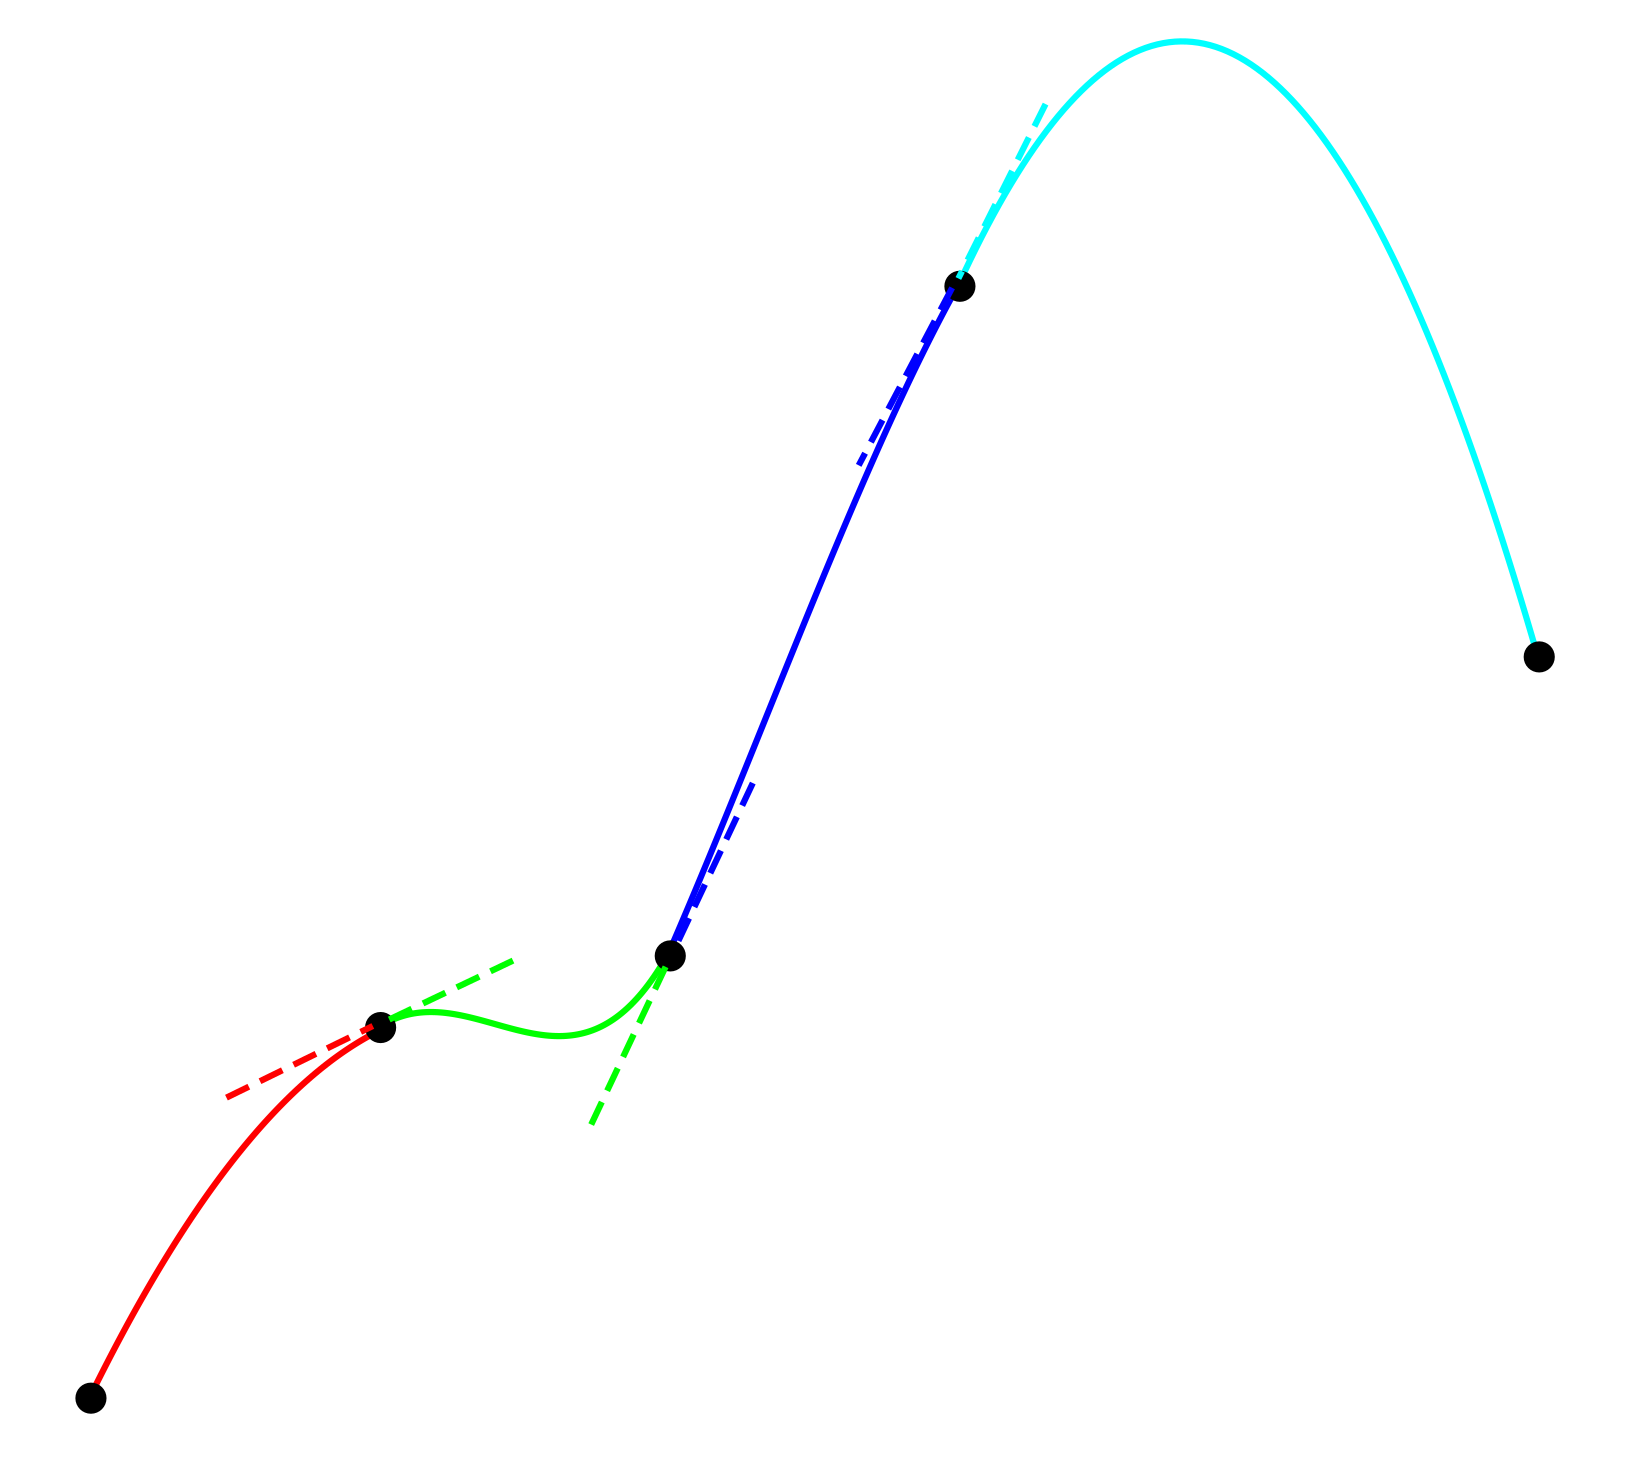
\includegraphics{new-spline.png}
	\end{center}
	\caption{Схематическое изображение аппроксимации сплайном, сплошная линии разных цветов --- полиномы составляющие сплайн, пунктирной линией показана касательная на границах }\label{fig:old.regress.spline}
\end{figure}

Для аппроксимация кубическим и параболическим сплайном в Mathcad есть встроенные функции \mc{cspline(x,y)} и \mc{pspline(x,y)} соответственно. Аргументами являются векторы исходных данных $x$ и $y$. В результате функция возвращает вектор, содержащий параметры полиномов в каждом из диапазонов. Для вычисления значения сплайн функции точке \mc{xt}, необходимо воспользоваться функцией \mc{interp(vs,x,y,xt)}.




\primer{Задайте произвольный набор данных \mc{x} и \mc{y} в виде таблицы. Для аппроксимации данных используете кубический сплайн и полином третьей степени. Постройте графики полученных функций и сравните результат.}
%пример решения
\begin{center}
	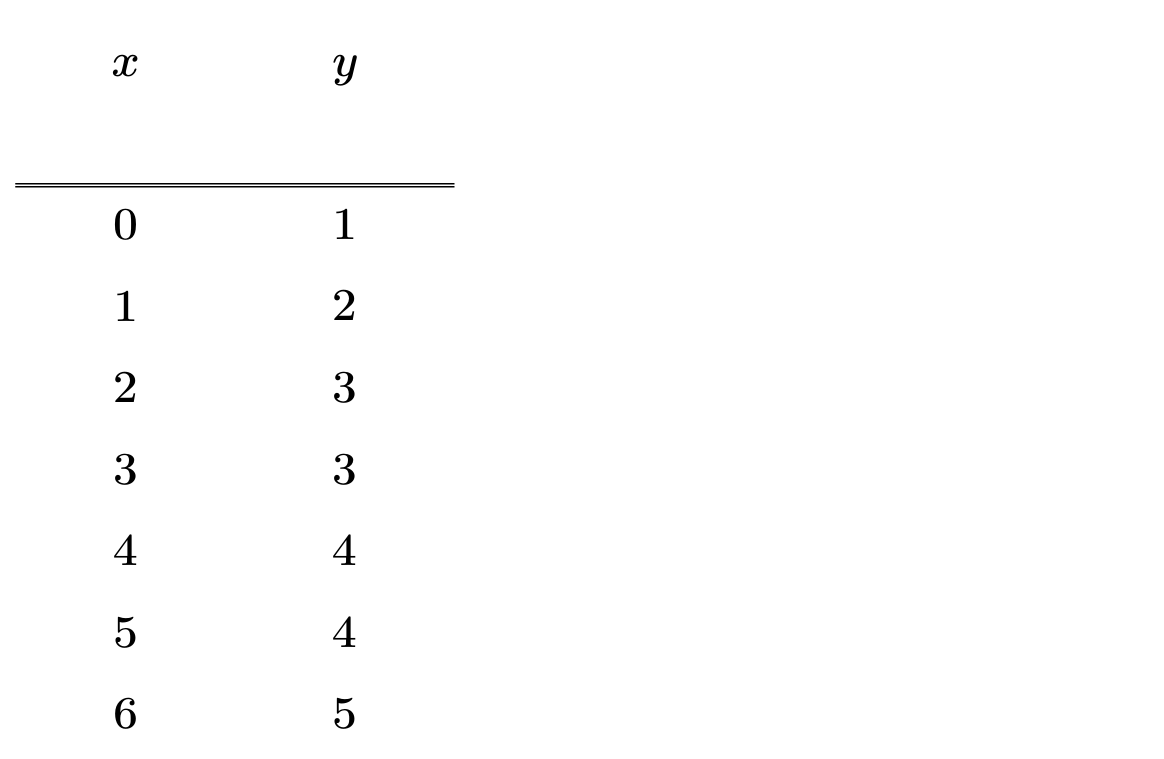
\includegraphics{new-regress-5-1.png}
\end{center}

\begin{center}
	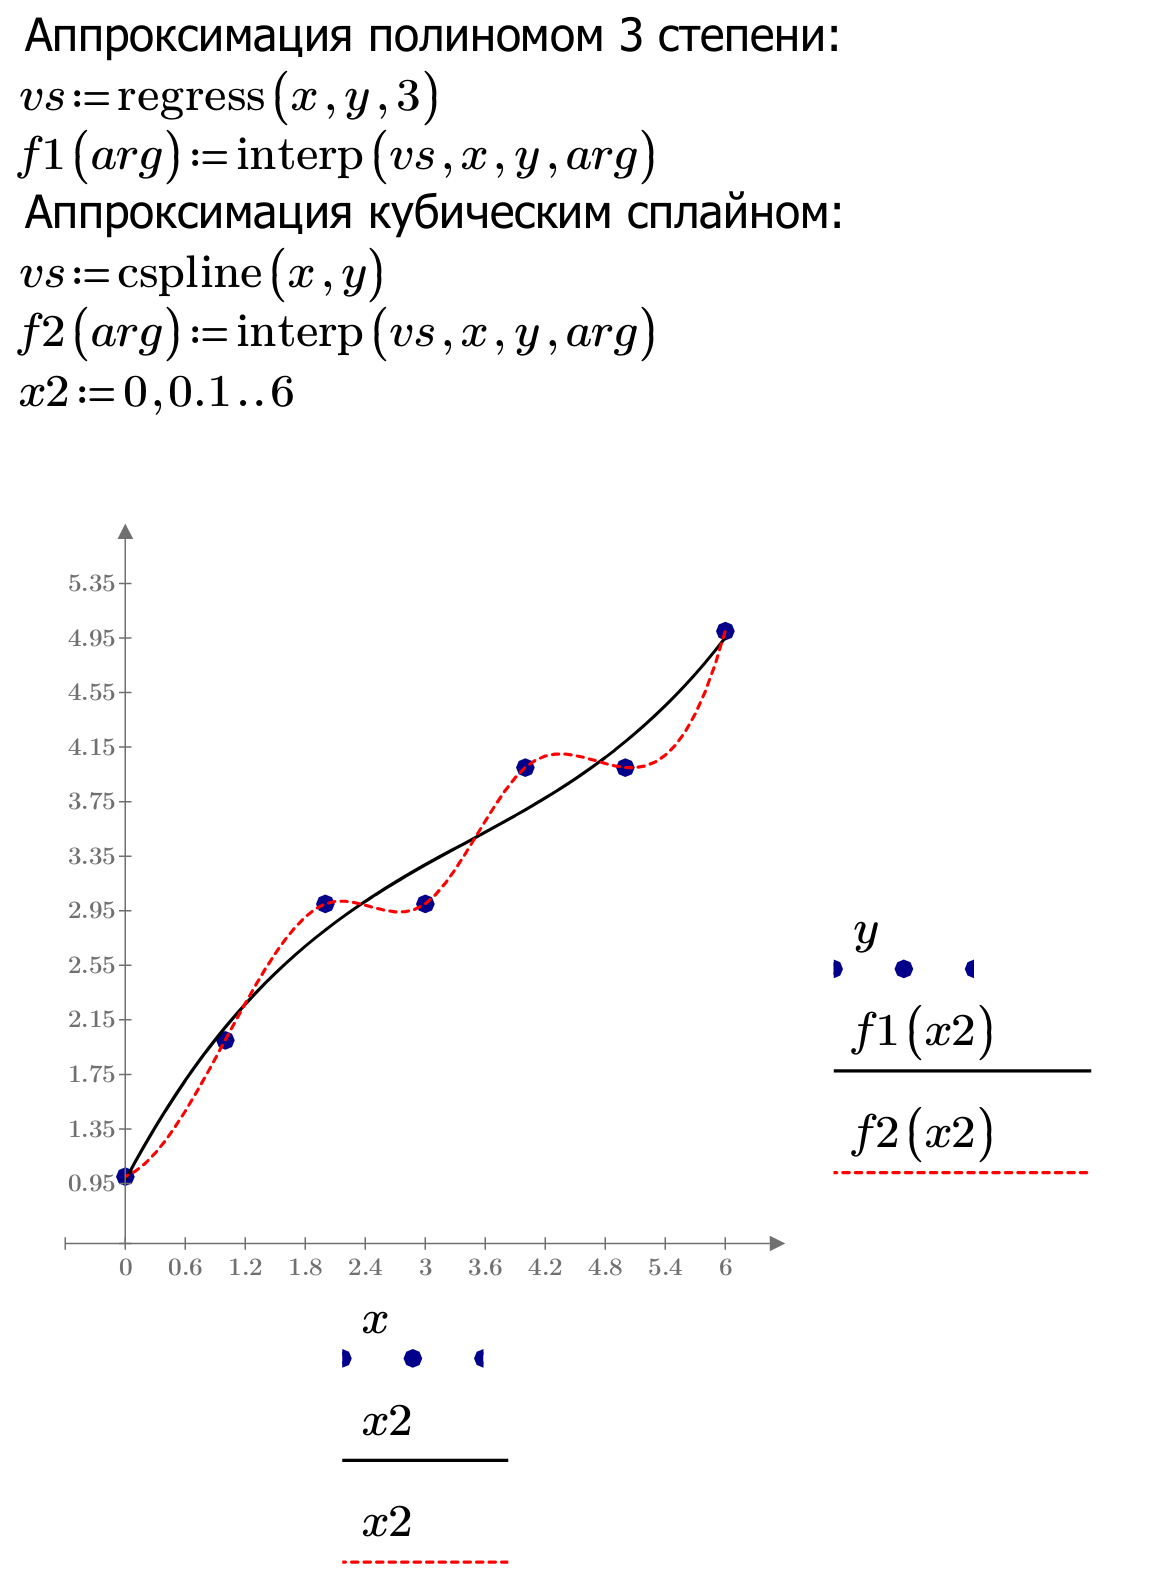
\includegraphics{new-regress-5-2.png}
\end{center}

Вопросы для самоконтроля:
\begin{enumerate}
	\item Что такое регрессионный анализ?
	\item Что такое коэффициент корреляции?
	\item Какие виды функций регрессии существуют, в чем их различие?
	\item Какие функции решения уравнения с одним неизвестным и системы уравнений используются в MathCad?
\end{enumerate}

\subsubsection*{Пример задания}
\begin{enumerate}
\item В результате измерения зависимости переменной состояния $y$ от входного фактора $x$ были получены значения, представленные в таблице. Описать табличные данные следующими функциональными зависимостями:
\begin{itemize} 
	\item $y(x)=a x+b$
	\item $y(x)=a_3 x^3 +a_2 x^2 + a_1 x +a_0$
	\item $y(x)=a e^{b x}+c  $
	\item $y(x)=a \cdot x^b+c$
	\item $y(x)=a_0 x                     +a_1 x^{3.7}                +a_2 \sqrt{x}              $
	\item $y(x)=A \cdot e^{-\dfrac{B}{x}+C}        $
	\item параболический сплайн
\end{itemize}
\begin{table}[h]
	\begin{tabular}{|c|c|}
		\hline
		x & y \\ \hline
		7.80 &     -62.58 \\ \hline 
		9.10 &    -116.08 \\ \hline 
		10.40 &    -157.64 \\ \hline 
		11.70 &    -143.06 \\ \hline 
		13.00 &    -257.91 \\ \hline 
		14.30 &    -386.64 \\ \hline 
		15.60 &    -323.30 \\ \hline 
	\end{tabular}
\end{table}

\item  Используя данные из справочника теплофизических свойств \cite{vargaftik} описать удельный объем изобутана при р = 1 атм изобутана. В качестве аппроксимирующей функции может выступать любое выражение, однако максимальное отклонение не должно превышать 10\%. Определить, при какой температуре удельный объем изобутана при р = 1 атм равен $   657.0 \frac {\text{дм}^3}{\text{кг}}$.
\end{enumerate}